% !TEX encoding = UTF-8
% !TEX TS-program = pdflatex
% !TEX root = ../tesi.tex
% !TEX spellcheck = it-IT

%**************************************************************
\chapter{Progettazione e codifica}
\label{cap:progettazione-codifica}
%**************************************************************

\intro{Breve introduzione al capitolo}\\

%**************************************************************

\section{Architettura di AngularJS}
AngularJS è stato il framework maggiormente utilizzato in questo stage e mi ha consentito di implementare l'intero progetto agilmente.\\
Alla base del framework, è collocato il design pattern \gls{mvc}, leggermente modificato per adattarsi alle funzionalità di AngularJS. Il design pattern che ne risulta è qualcosa di più flessibile del classico \gls{mvc}, consentendo agli sviluppatori una maggior libertà di utilizzo.\\
Ovviamente ci sono delle direttive e delle \emph{best practice} consigliate, soprattutto se si intende creare un \gls{front-end} davvero \gls{rest}-ful.

\subsection{Model}
In AngularJS, il "`\emph{model}"' è realizzato con precise strutture dati. Innanzitutto, la logica di business dell'applicazione si colloca nei cosiddetti \emph{servizi}. I servizi sono dei \emph{singleton} istanziati con tecnica \emph{lazy}, ovvero alla prima invocazione. In queste strutture è collocata tutta la logica che è indipendente dalla \emph{view}, puntando al suo massimo riutilizzo.\\
Differentemente dai controller, le \emph{Factory} dei servizi vengono richiamate dal sistema di \emph{Dependendcy Injection}. Questo avviene passando come argomento al construttore di una struttura il nome del servizio da richiamare; sarà poi compito dell'\emph{injector} di AngularJS richiamare la corretta \emph{factory} del servizio richiesto.\\
I servizi vegono utilizzati inoltre (e soprattutto) per gestire i dati sensibili dell'utenza e dei vari oggetti presenti nel \gls{back-end}. Sono loro, infatti, gli esecutori materiali delle richieste \gls{rest} al \gls{back-end}, grazie alle direttive apposite, come \textbf{\$http} e \textbf{\$resource}; i dati risultanti verranno poi forniti alle viste, se necessario, passando per gli adeguati controller.

\begin{figure}[!h] 
    \centering 
    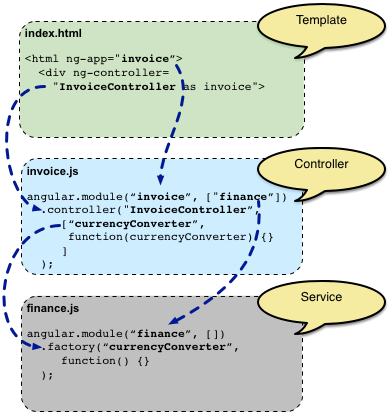
\includegraphics[width=0.7\columnwidth]{concepts-module-service} 
    \caption{Esempio di legame tra vista-controller-servizio}
\end{figure}

\subsection{View}
Le viste realizzate con AngularJS sono essenzialmente pagine web con delle funzionalità di \emph{markup} aggiuntive. All'interno di una pagina scritta in codice \gls{html}, si possono utilizzare delle direttive di AngularJS che verranno interpretate prima di renderizzare la pagina. Tramite queste direttive è possibile visualizzare dati del modello, modificarli in \emph{real time} grazie al \emph{Two-way data binding} richiamare funzioni di uno specifico controller e molto altro.\\
La classica dicitura di AngularJS per identificare un'espressione da interpretare si ottiene racchiudendo l'espressione tra due parentesi graffe: 
\begin{verbatim}
{{ espressione }}
\end{verbatim}
All'interno di questa dicitura, ogni espressione viene valutata e il suo risultato viene renderizzato nella pagina web. Se, ad esempio, nel \emph{template} \gls{html} si inserisce un'operazione matematica all'interno delle doppie graffe, una volta renderizzata la pagina il risultato dell'operazione (se possibile) verrà mostrato al posto dell'espressione.\\
Oltre a questa funzionalità, AngularJS mette a disposizione una grande varietà di direttive per manipolare il \gls{dom}, come iteratori per scorrere insiemi di dati o filtri da applicare ad una collezione per limitarne la visualizzazione.

\begin{figure}[!h] 
    \centering 
    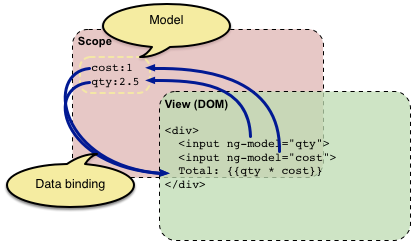
\includegraphics[width=0.9\columnwidth]{concepts-databinding1} 
    \caption{Esempio di Template di una vista e Data Binding}
\end{figure}

\subsection{Controller}
I controller in AngularJS sono ciò che implementa la logica applicativa. Vengono legati al \emph{template} di una pagina tramite la direttiva \textbf{ng-controller} posta all'interno di un elemento \gls{html}. Così facendo, si invoca il costruttore del controller designato; lo \emph{scope} del controller appena creato è l'elemento in cui è stato dichiarato e gli eventuali nodi figli dell'elemento stesso.\\
Il principale scopo dei controller è di esporre funzionalità alle espressioni ed alle direttive utilizzate all'interno delle pagine web. Questo si ottiene aggiungendo metodi e proprietà all'oggetto \textbf{\$scope} che verrà condiviso con la vista. Questo oggetto in particolare permette di realizzare il cosiddetto \emph{view-model}, ovvero quella parte del \emph{model} che verrà presentata alla \emph{view}. Inoltre, tutte le proprietà associate al controller saranno rese disponibili al \emph{template}, nello \emph{scope} che compete al controller.

\begin{figure}[!h] 
    \centering 
    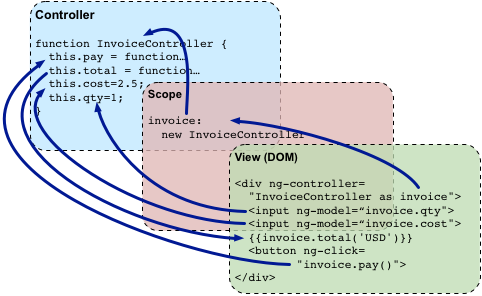
\includegraphics[width=0.75\columnwidth]{concepts-databinding2} 
    \caption{Esempio di legame tra template e Controller}
\end{figure}

\subsection{Two-way Data Binding}
Una funzionalità importante che AngularJS espone è il cosiddetto \emph{Two Way Data Binding}. Si parla di \emph{legame doppio tra dati} quando una variabile del modello è legata ad un elemento che può cambiare ed al contempo mostrare il contenuto della variabile stessa. In una vista di AngularJS, ogniqualvolta un elemento che applica il \emph{Two Way Data Binding} viene modificato, il corrispondente campo nel modello viene notificato e aggiornato correttamente.\\
In AngularJS, si usa la direttiva \textbf{ng-model} per legare una variabile del modello ad un elemento \gls{html} che può sia mostrare il suo valore, che modificarlo.

\begin{figure}[H] 
    \centering 
    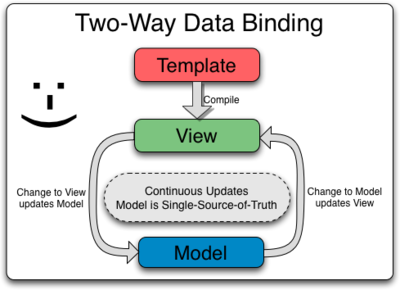
\includegraphics[width=0.8\columnwidth]{two_way_data_binding} 
    \caption{Doppio legame tra vista e modello di AngularJS}
\end{figure}

\subsection{Dependency Injection}
\emph{Dependency Injection} è un design pattern creato per gestire e risolvere le varie dipendenze tra più moduli software, e viene utilizzato all'interno di questo particale \emph{framework} JavaScript.\\
La responsabilità di fornire le varie componenti richieste dalle dipendenze è demandata al sottosistema di gestione delle iniziezioni di AngularJS. Ogni volta che si dichiara una componente, viene registrata al modulo corrispondente; in questo modo, il sistema di gestione delle dipendenze può riconoscere la componente ed usarla dove è richiesto.\\
Quando è richiesta una dipendenza, l'iniettore controlla il nome con cui è stata richiesta e la cerca nelle dipendenze registrate nel modulo, per iniettarla dove richiesto, se presente.

\begin{figure}[!h] 
    \centering 
    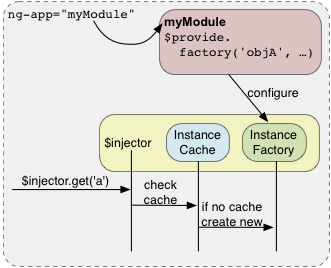
\includegraphics[width=0.7\columnwidth]{concepts-module-injector} 
    \caption{Esempio di configurazione di una factory per l'iniettore}
\end{figure}

%**************************************************************

\section{Definizione delle API REST}
Questa sezione presenta la lista delle \gls{api} concordate per le richieste \gls{rest} al \gls{back-end}. Ogni definizione comprende l'\gls{uri} di riferimento, il tipo di richiesta e i valori di ritorno possibili.\\
Nelle \gls{uri} delle richieste, la dicitura \textbf{vx} sta ad indicare il numero di versione della richiesta, mentre l'espressione \textbf{:variabile} sta ad indicare una porzione variabile dell'\gls{uri}, utilizzata da AngularJS.

\subsection{Informazioni utente}

\subsubsection{Lettura}

\paragraph{URL}
/api/vx/users/:username
\paragraph{Metodo}
GET
\paragraph{Contenuto della richiesta}
nessuno
\paragraph{Risposte}
\begin{itemize}
	\item[200] la risposta contiene il \gls{json} compatto con le proprietà utente;
	\item[404] se l'utente non è presente;
	\item[403] se l'utente non è autorizzato ad accedere all'informazione.
\end{itemize}


\subsubsection{Invio di dati per l'autenticazione}
\paragraph{URL}
/api/vx/login
\paragraph{Metodo}
POST
\paragraph{Contenuto della richiesta}
file \gls{json} con la seguente formattazione:
\begin{verbatim}
{
  'username': 'some_username',
  'password': 'some_password'
}
\end{verbatim}
\paragraph{Risposte}
\begin{itemize}
	\item[200] la risposta contiene il \gls{json} compatto con le proprietà utente, più un \emph{token} utilizzato per comporre l'\emph{header} di autenticazione;
	\item[400] se gli \emph{header} sono invalidi oppure se il contenuto della richiesta non è corretto;
	\item[403] se l'autenticazione non è andata a buon fine.
\end{itemize}

\subsubsection{Creazione di un nuovo utente}
\paragraph{URL}
/api/vx/users
\paragraph{Metodo}
PUT
\paragraph{Contenuto della richiesta}
file \gls{json} compatto contenente username ed email
\paragraph{Risposte}
\begin{itemize}
	\item[201] la risposta contiene l'\emph{id} della proprietà creata;
	\item[400] se gli \emph{header} sono invalidi oppure se il contenuto della richiesta non è corretto;
	\item[403] se l'utente non è autorizzato alla creazione di un nuovo utente.
\end{itemize}

\subsubsection{Modifica dei dati utente}
\paragraph{URL}
/api/vx/users/:username
\paragraph{Metodo}
PATCH
\paragraph{Contenuto della richiesta}
file \gls{json} contenente le modifiche da applicare all'utente designato
\paragraph{Risposte}
\begin{itemize}
	\item[204] corpo vuoto;
	\item[400] se gli \emph{header} sono invalidi oppure se il contenuto della richiesta non è corretto;
	\item[403] se l'utente non è autorizzato a modificare l'entità.
\end{itemize}

\subsection{Esperienze professionali}

\subsubsection{Lettura}
\paragraph{URL}
/api/vx/users/:username/experiences
\paragraph{Metodo}
GET
\paragraph{Contenuto della richiesta}
nessuno
\paragraph{Risposte}
\begin{itemize}
	\item[200] la risposta contiene il \gls{json} con l'\emph{array} di esperienze;
	\item[404] se la risorsa non è presente;
	\item[403] se l'utente non è autorizzato ad accedere all'informazione.
\end{itemize}


\subsubsection{Inserimento di una nuova esperienza}
\paragraph{URL}
/api/vx/users/:username/experiences
\paragraph{Metodo}
PUT
\paragraph{Contenuto della richiesta}
file \gls{json} con la seguente formattazione:
\begin{verbatim}
{
  'role': 'ruolo_aziendale',
  'company': 'nome_azienda',
  'managerName': 'nome_responsabile',
  'managerMail': 'mail_responsabile',
  'beginDate': 'data_ISO',
  'endDate': 'data_ISO',
  'description': "breve descrizione dell'esperienza lavorativa",
  'area': 'area_competenza',
  'technologies': 'stack_utilizzati'
}
\end{verbatim}
\paragraph{Risposte}
\begin{itemize}
	\item[201] la risposta contiene il \gls{json} dell'esperienza appena creata;
	\item[400] se gli \emph{header} sono invalidi oppure se il contenuto della richiesta non è corretto;
	\item[403] se l'utente non è autorizzato a creare una nuova esperienza.
\end{itemize}

\subsubsection{Modifica dei dati di un'esperienza}
\paragraph{URL}
/api/vx/users/:username/esperiences/:experience
\paragraph{Metodo}
PATCH
\paragraph{Contenuto della richiesta}
file \gls{json} contenente le modifiche da applicare all'esperienza dell'utente
\paragraph{Risposte}
\begin{itemize}
	\item[204] corpo vuoto;
	\item[400] se gli \emph{header} sono invalidi oppure se il contenuto della richiesta non è corretto;
	\item[403] se l'utente non è autorizzato a modificare l'entità.
\end{itemize}


\subsection{Titoli di studio ed abilitazioni professionali}

\subsubsection{Lettura}
\paragraph{URL}
/api/vx/users/:username/qualifications
\paragraph{Metodo}
GET
\paragraph{Contenuto della richiesta}
nessuno
\paragraph{Risposte}
\begin{itemize}
	\item[200] la risposta contiene il \gls{json} con l'\emph{array} di qualificazioni;
	\item[404] se la risorsa non è presente;
	\item[403] se l'utente non è autorizzato ad accedere all'informazione.
\end{itemize}


\subsubsection{Inserimento di una nuova qualificazione}
\paragraph{URL}
/api/vx/users/:username/qualifications
\paragraph{Metodo}
PUT
\paragraph{Contenuto della richiesta}
file \gls{json} con una tra le seguenti formattazioni:
\begin{itemize}
\item se la qualificazione in questione non è un \emph{workshop}, ovvero non è un prodotto:
\begin{verbatim}
{
  'type': 'tipo_certificazione',
  'authority': 'ente_di_rilascio',
  'address': 'recapito_ente',
  'grade': 'grado_certificazione',
  'earnDate': 'data_ISO'
}
\end{verbatim}
\item se la qualificazione in questione è un \emph{workshop}:
\begin{verbatim}
{
  'type': 'workshop',
  'authority': 'ente_di_rilascio',
  'address': 'recapito_ente',
  'grade': 'grado_certificazione',
  'earnDate': 'data_ISO',
  'vendor': 'committente',
  'product': 'nome_workshop',
  'expireDate': 'data_ISO'
}
\end{verbatim}
\end{itemize}
\paragraph{Risposte}
\begin{itemize}
	\item[201] la risposta contiene il \gls{json} della qualificazione appena creata;
	\item[400] se gli \emph{header} sono invalidi oppure se il contenuto della richiesta non è corretto;
	\item[403] se l'utente non è autorizzato a creare una nuova qualificazione.
\end{itemize}

\subsubsection{Modifica dei dati di una qualificazione}
\paragraph{URL}
/api/vx/users/:username/qualifications/:qualification
\paragraph{Metodo}
PATCH
\paragraph{Contenuto della richiesta}
file \gls{json} contenente le modifiche da applicare alla qualificazione dell'utente
\paragraph{Risposte}
\begin{itemize}
	\item[204] corpo vuoto;
	\item[400] se gli \emph{header} sono invalidi oppure se il contenuto della richiesta non è corretto;
	\item[403] se l'utente non è autorizzato a modificare l'entità.
\end{itemize}

\subsection{Skill}

\subsubsection{Lettura}
\paragraph{URL}
/api/vx/users/:username/experiences
\paragraph{Metodo}
GET
\paragraph{Contenuto della richiesta}
nessuno
\paragraph{Risposte}
\begin{itemize}
	\item[200] la risposta contiene il \gls{json} con l'\emph{array} di esperienze;
	\item[404] se la risorsa non è presente;
	\item[403] se l'utente non è autorizzato ad accedere all'informazione.
\end{itemize}


\subsubsection{Inserimento di una nuova esperienza}
\paragraph{URL}
/api/vx/users/:username/experiences
\paragraph{Metodo}
PUT
\paragraph{Contenuto della richiesta}
file \gls{json} con la seguente formattazione:
\begin{verbatim}
{
  'role': 'ruolo_aziendale',
  'company': 'nome_azienda',
  'managerName': 'nome_responsabile',
  'managerMail': 'mail_responsabile',
  'beginDate': 'data_ISO',
  'endDate': 'data_ISO',
  'description': "breve descrizione dell'esperienza lavorativa",
  'area': 'area_competenza',
  'technologies': 'stack_utilizzati'
}
\end{verbatim}
\paragraph{Risposte}
\begin{itemize}
	\item[201] la risposta contiene il \gls{json} dell'esperienza appena creata;
	\item[400] se gli \emph{header} sono invalidi oppure se il contenuto della richiesta non è corretto;
	\item[403] se l'utente non è autorizzato a creare una nuova esperienza.
\end{itemize}

\subsubsection{Modifica dei dati di un'esperienza}
\paragraph{URL}
/api/vx/users/:username/esperiences/:experience
\paragraph{Metodo}
PATCH
\paragraph{Contenuto della richiesta}
file \gls{json} contenente le modifiche da applicare all'esperienza dell'utente
\paragraph{Risposte}
\begin{itemize}
	\item[204] corpo vuoto;
	\item[400] se gli \emph{header} sono invalidi oppure se il contenuto della richiesta non è corretto;
	\item[403] se l'utente non è autorizzato a modificare l'entità.
\end{itemize}

\subsection{Progetti associati}

%**************************************************************


\section{Stub Back-end}
Il progetto di stage ha avuto come oggetto la realizzazione di un \gls{front-end} gestionale, senza però avere al contempo un \gls{back-end} funzionante. Per le verifiche funzionali, quindi, ho avuto bisogno di realizzare un \gls{back-end} fittizio, il quale mi consentisse di effettuare chiamate alle \gls{api} concordate con il Responsabile di Progetto per il \gls{back-end} vero e proprio.\\
Per realizzare questo \gls{back-end} sono ricorso a delle feature fornite dalle librerie di AngularJS adibite al testing di unità. Durante il testing delle funzionalità di una componente, le richieste ad un server funzionante vengono sostituite con una chiamata ad hoc che deve rispettare certe precondizioni e che restituisce dei dati prestabiliti. Il concetto del \gls{back-end} di \gls{stub} che ho utilizzato è lo stesso. In particolare, grazie all'utilizzo di espressioni regolari per filtrare le chiamate \gls{rest}, sono stato in grado di intercettare tali chiamate e di farle gestire al mio \gls{back-end} ad hoc, con risposte prestabilite.\\
Tutto ciò è stato possibile gran parte grazie al servizio \textbf{\$httpBackend} di AngularJS, il quale contiene metodi di intercettazione di chiamate \gls{rest} e di gestione di richieste e risposte (e relativi \emph{header}) \gls{http}. Il frammento sottostante è un esempio di una chiamata \gls{http} gestita dal \gls{back-end} di \gls{stub}:

\begin{verbatim}
$httpBackend.whenGET(/\/api\/\d.\d\/users\/\w*\/qualification/).respond(function(method, url, data, headers) {
  console.log('Received these data:', method, url, data, headers);
  var getStatus,
   getData = {},
   getHeaders = headers;
  if(headers.Authorization == "Bearer XXX") {
    getStatus = 200;
    getData = {
      qualifications: [
        {
          type: 'Workshop',
          authority: 'W3C',
          address: 'Silicon Valley, 42',
          grade: 'Senior',
          earnDate: new Date(2015, 4, 20).toISOString(),
          vendor: 'RFC',
          product: 'HTML6',
          expireDate: new Date(2050, 4, 20).toISOString()
        },
        {
          type: 'Certificazione',
          authority: 'Mongo',
          address: 'MongoDB avenue, 8080',
          grade: 'Senior',
          earnDate: new Date(2014, 7, 8).toISOString()
        },
        {
          type: 'Corso',
          authority: 'AngularJS',
          address: '1600 Amphitheatre Parkway Mountain View, CA 94043',
          grade: 'Junior',
          earnDate: new Date(2015, 5, 20).toISOString()
        }
      ]
    };
  }
  else
    getStatus = 401;
  return [getStatus, getData, getHeaders];
});
\end{verbatim} 
%Oltre a permettermi di controllare l'effettivo funzionamento dell'applicazione, un \gls{backend} di %questo tipo mi consente inoltre di verificare 

%**************************************************************

\section{Tecnologie e strumenti}
\label{sec:tecnologie-strumenti}

Di seguito viene data una panoramica delle tecnologie e strumenti utilizzati.

\subsection*{Tecnologia 1}
Descrizione Tecnologia 1.

\subsection*{Tecnologia 2}
Descrizione Tecnologia 2

%**************************************************************
\section{Ciclo di vita del software}
\label{sec:ciclo-vita-software}

%**************************************************************
\section{Progettazione}
\label{sec:progettazione}

\subsubsection{Namespace 1} %**************************
Descrizione namespace 1.

\begin{namespacedesc}
    \classdesc{Classe 1}{Descrizione classe 1}
    \classdesc{Classe 2}{Descrizione classe 2}
\end{namespacedesc}


%**************************************************************
\section{Design Pattern utilizzati}

%**************************************************************
\section{Codifica}
